\section{Ablation and Sensitivity}\label{sec:ablation}
\textbf{E4: component ablations.} Five variants were run on all 321 pairs through configuration deltas (Table~\ref{tab:e4}): V1 $r_{det}=1$, V2 $r_{replay}=1$, V3 $k_{alt}=0$, V4 all three, V5 the fd-1 stdout fold off. \textbf{No variant changes the verdict value or level on any of the 321 pairs}; detection, false assurance, abstention and false alarm are identical and all paired $p$-values are 1.0 (no discordant pairs). The only observable difference is one reason code: \texttt{black\_\_21\_\_black\_py\_\_dump\_to\_file} moves from \texttt{nondeterministic} to \texttt{flaky\_witness} under V1 and V4 (both \INS{}). Witness ids change under V2--V4 because the replay set is part of the witness (84 pairs). V0 equals E3 on 320 of 321 strict keys; the exception is explained in Section~\ref{sec:failure}.
\begin{table}[t]\centering\scriptsize\setlength{\tabcolsep}{3pt}
\caption{E4 ablations on the 321 pairs (verdict counts; flips = pairs whose verdict value or level differs from V0). CPU is the summed per-pair CPU of the run (concurrency 4, load-sensitive). Only a reason code changes (one pair, V1 and V4). Source: \path{results/v7b_phase2_summary/p2_consolidated_20261118_190644/consolidated.json}, key \texttt{E4}.}\label{tab:e4}
\resizebox{\linewidth}{!}{%
\begin{tabular}{llrrrrr}
\hline
Variant & Change & DIV & INSUF. & NDO & Flips vs V0 & CPU s (sum) \\
\hline
V0 & default & 84 & 157 & 71 & -- & 546.8 \\
V1 & $r_{det}=1$ & 84 & 157 & 71 & 0 & 271.6 \\
V2 & $r_{replay}=1$ & 84 & 157 & 71 & 0 & 521.4 \\
V3 & $k_{alt}=0$ & 84 & 157 & 71 & 0 & 512.5 \\
V4 & V1+V2+V3 & 84 & 157 & 71 & 0 & 225.1 \\
V5 & FOLD\_FD1=False & 84 & 157 & 71 & 0 & 520.1 \\
\hline
\end{tabular}}
\end{table}

\textbf{Interpretation limit.} The dataset contains almost no intermittent or control-sensitive behaviour (E1: 1 of 312 pairs quarantined), so the confirmation machinery has nothing to filter. The experiment can show a cost (V4 uses about 65\% fewer runs, 4,746 versus 13,764 run records, for the same verdicts here) but \textbf{it cannot show the value of the components, and component importance must not be inferred}. The B1 versus B1+rep result (identical on all primary outcomes) points the same way and is equally uninformative about data containing real flakiness. Hash-order sensitivity is untested.

\textbf{E5: S2 branch-coverage floor.} The floor was run at 0.6, 0.8 (default) and 0.9 separately (Fig.~\ref{fig:e5}). Verdict values are identical at all floors (0 value flips); the NO\_DIVERGENCE\_OBSERVED pairs split 71/0, 55/16 and 43/28 between S2 and S1 (monotone, as pre-registered), 16 pairs change S1/S2 label between 0.6 and 0.8 and 12 between 0.8 and 0.9. Detection (0.708), false assurance (0.123) and abstention (0.473) are identical at all floors, so the pre-registered ``headline stable'' criterion holds. The floor does not change whether a verdict is issued, only the S1/S2 label; the stability is a property of the decision rule, not evidence that 0.8 is well chosen, and no threshold was selected retrospectively.
\begin{figure}[t]\centering
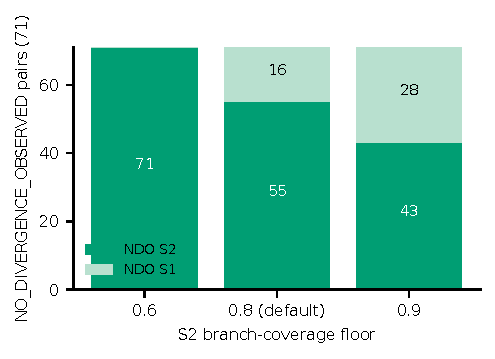
\includegraphics[width=0.92\columnwidth]{../../results/v7b_phase2_summary/figures/fig_p2_e5_floors.pdf}
\caption{E5: share of NO\_DIVERGENCE\_OBSERVED pairs labelled S2 versus S1 as the S2 branch floor varies. Verdict values are unchanged. Source: \path{results/v7b_phase2_summary/p2_consolidated_20261118_190644/consolidated.json}, key \texttt{E5}.}\label{fig:e5}
\end{figure}

\textbf{Other sensitivity and generalisation.} Repeat counts, the CPU budget and the per-run limits were not varied. Nothing supports generalisation across projects, domains, languages or platforms (Section~\ref{sec:limitations}).
